\def\QRCODE{TB_IPR_TUT.IMG.stereology_pythonqrcode.png}
\def\QRPAGE{http://www.iptutorials.science/tree/master/TB_IPR/TUT.IMG.stereology/python}
\pcorrectionsection{Python correction}

\begin{python}
import numpy as np
import matplotlib.pyplot as plt
import skimage.measure
import scipy
\end{python}

\subsection{Classical measurements of stereology}

To generate a binary image with overlapping random disks (see Fig.\ref{fig:stereology:python:disks}), the following function is used:
\begin{python}
def popDisks(nb_disks, S, Rmax):
    """ Generates an image with random disks, with uniform distribution of the centers, and of the radii.
    @param nb_disks: number of disks
    @type S: int
    @param S: Size of spatial support
    @param rmax: maximum radius of disks
    @return: binary image of disks
    """
    centers = np.random.randint(S, size=(nb_disks,2));
    radii = Rmax * np.random.rand(nb_disks);
    
    N=1000;
    x = np.linspace(0, S, 1000);
    y = np.linspace(0, S, 1000);
    X, Y = np.meshgrid(x, y);
    I = np.zeros((N,N));
    for i in range(nb_disks):
        I2 = (X-centers[i,0])**2 + (Y-centers[i,1])** 2 <= radii[i]**2;
        I = np.logical_or(I, I2);
        
    return I;
\end{python}

\begin{figure}[htbp]
 \centering\caption{Random population of disks.}%
 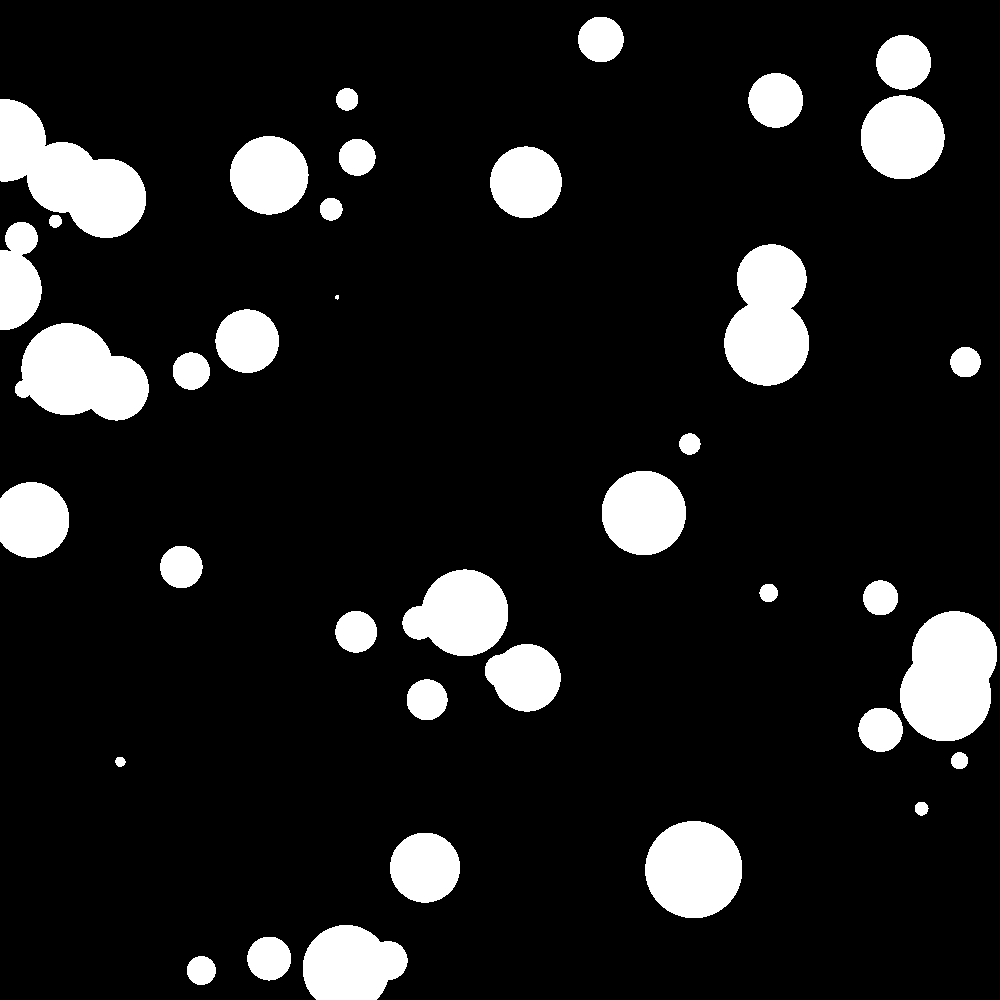
\includegraphics[width=.3\textwidth]{disques.png}%
 \label{fig:stereology:python:disks}%
\end{figure}

\subsubsection{Area fraction}
The area fraction counts the number of probes that lay inside the objects. In order to verify this probe, the next function evaluates the real area covered by the disks.
\begin{python}
def areaFraction(nb_probes, I):
    """
    Evaluates area fraction via point probes
    @param nb_probes: number of probes
    @param I: binary image, square
    """
    P = np.random.randint(I.shape[0], size = (nb_probes,2));

    # count the number of probes in phase
    count = np.sum(I[P[:,0], P[:,1]]);
    return float(count) / nb_probes;
\end{python}

\begin{python}
def verifyAreaFraction():
    """
    Verify area fraction
    """
    I = popDisks(50, 1000, 20);
    plt.imshow(I);
    AA = float(np.sum(I)) / np.size(I);
    PP = areaFraction(3000, I);

    print("AA (true number of pixels): {:.2%}".format(AA));
    print("PP (evaluated fraction)   : {:.2%}".format(PP));      
\end{python}

There is a good agreement between $AA$ and $PP$. The method is illustrated in Fig.\ref{fig:stereology:python:areafraction}.

\begin{figure}[htbp]
 \centering\caption{Illustration of the positions of the different probes.}%
 \subfloat[Area fraction evaluation.]{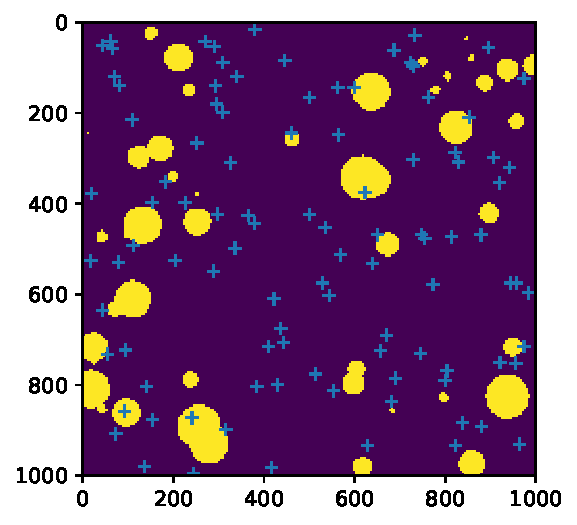
\includegraphics[width=.45\linewidth]{areaFrac.pdf}\label{fig:stereology:python:areafraction}}\hfill
 \subfloat[Length per area evaluation.]{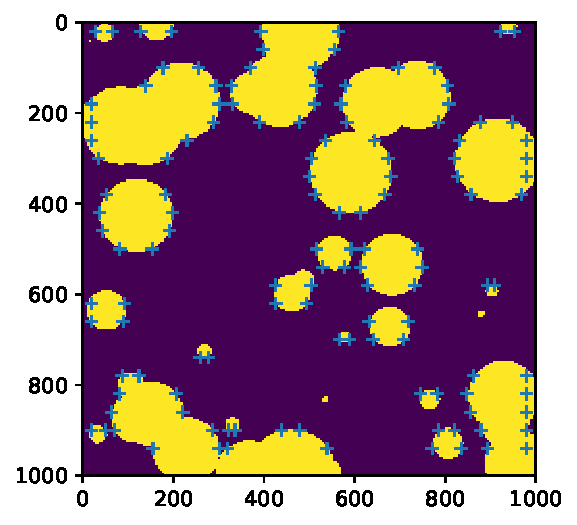
\includegraphics[width=.45\linewidth]{lengthPerArea.pdf}\label{fig:stereology:python:lengthperarea}}%
 \label{fig:stereology:python:fractions}%
\end{figure}


\begin{sh}
AA (true number of pixels): 2.05%
PP (evaluated fraction)   : 1.87%
\end{sh}

\subsubsection{Length per area}
A certain number of segments are used in order to perform the probing. The number of times a segment goes through the surface of the object is evaluated. This is illustrated in Fig.\ref{fig:stereology:python:lengthperarea}.

\begin{python}
def lengthPerArea(I):
    """
    Evaluates the length per area
    """
    perim= skimage.measure.perimeter(I.astype(int), 8);
    LA = perim / np.sum(I);
    print("LA (true count): {:.2%}".format(LA));
    
    # lines probes, every 10 pixels
    probe = np.zeros(I.shape);
    probe[20:-20:10, 20:-20] = 1;
    lines = I.astype(int) * probe;
    
    # count number of intercepts
    h = np.array([[1, -1, 0]]);    
    points = scipy.signal.convolve2d(lines, h, mode='same');

    nb_lines = np.sum(lines);
    nb_points= np.sum(np.abs(points));
    PL = float(nb_points) / nb_lines;
    print("pi/2*PL (true count): {:.2%}".format(np.pi/2*PL));
\end{python}

\begin{python}
def verifyLengthPerArea():
    I = popDisks(50, 1000, 20);
    plt.imshow(I);
    plt.show();
    lengthPerArea(I);
\end{python}

The perimeter evaluation may vary a lot according to the implementations or to the connectivity chosen.
\begin{sh}
LA (true count): 18.02%
pi/2*PL (evaluated fraction): 15.20%
\end{sh}

\subsubsection{Volume fraction}
This example loads a \matlabregistered{} matrix.

\begin{python}
def volumeFraction(volume):
    """
    """  
    VV = float(np.sum(volume)) / np.size(volume);
    probe= np.zeros(volume.shape);
    probe[10:-10:50, 10:, 10:] = 1;
    
    s = np.sum(probe);
    probe = probe * volume;
    AA = float(np.sum(probe)) / s;
    
    print("VV (true count): {:.2%}".format(VV));
    print("AA (true count): {:.2%}".format(AA));
    
def verifyVolumeFraction():
    sphere = scipy.io.loadmat("spheres.mat");
    volumeFraction(sphere['A']);
\end{python}

\begin{figure}[htbp]
 \centering\caption{Random population of 3D overlapping spheres. This function uses povray and the vapory python API.}%
 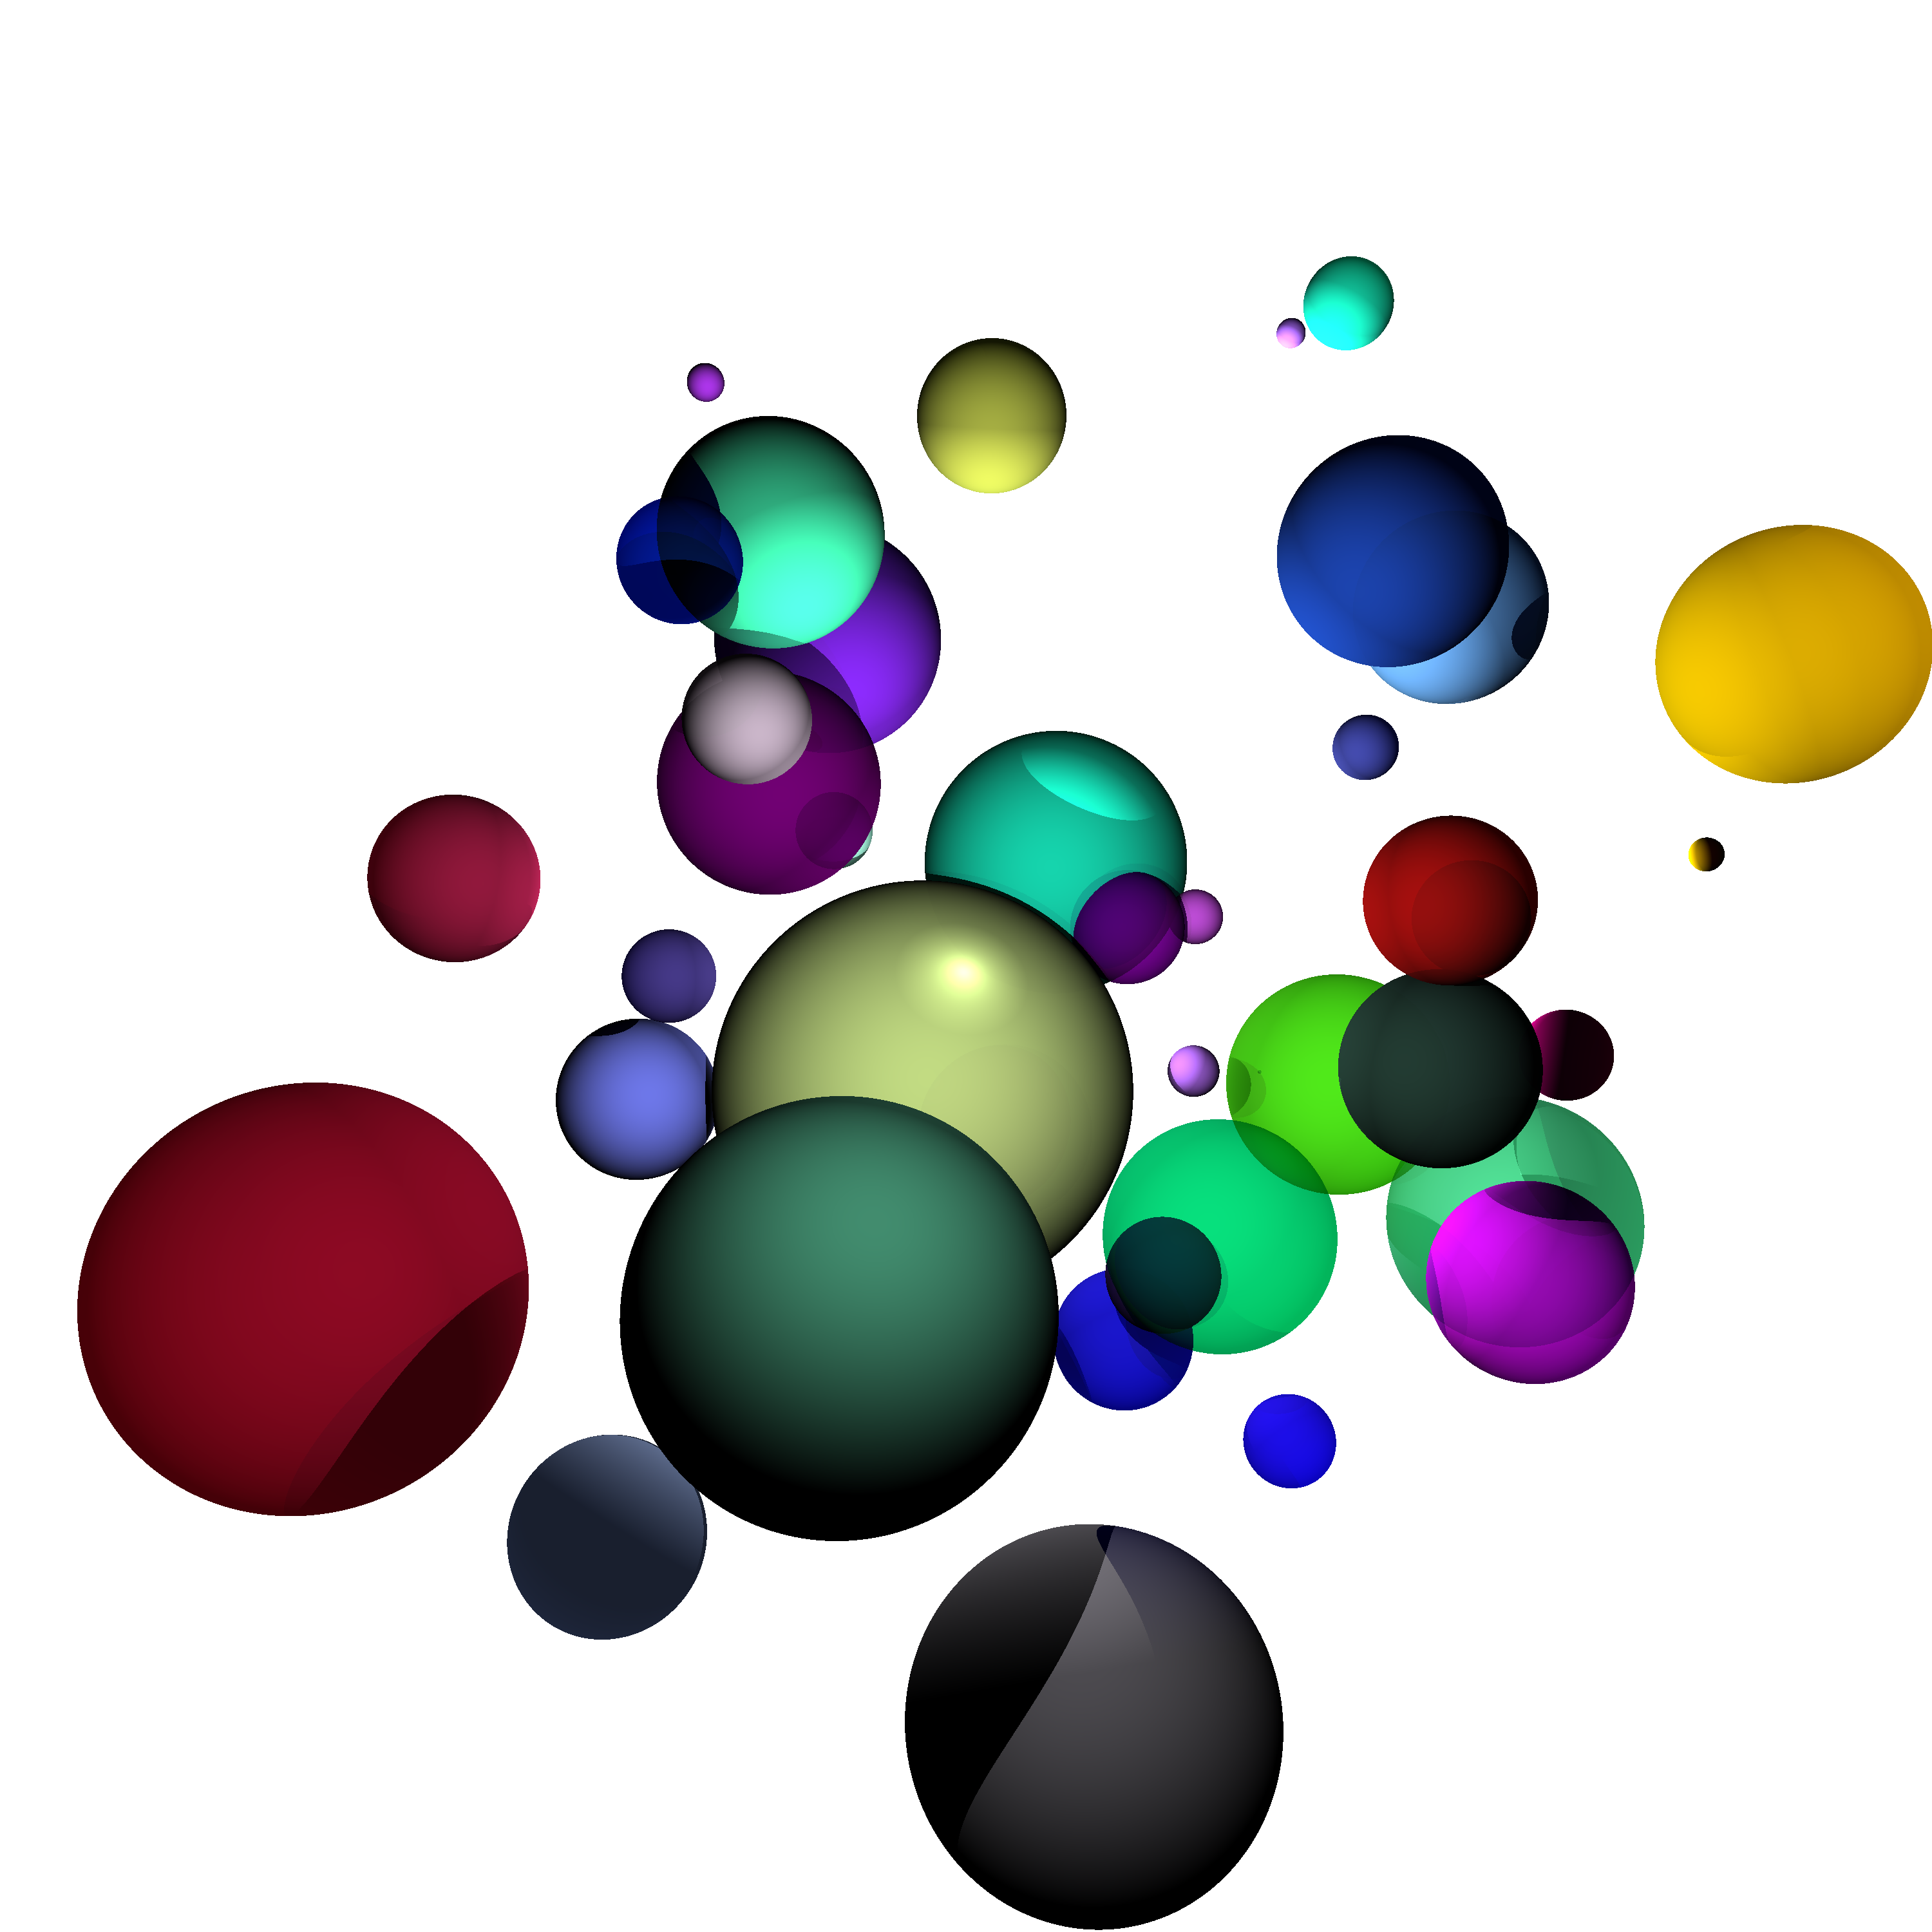
\includegraphics[width=9cm]{spheres.png}%
 \label{fig:stereology:python:overlapping_spheres}%
\end{figure}

As for the area fraction, the volume fraction is precise. The results on this example are:

\begin{sh}
VV (true count): 5.02%
AA (evaluated fraction): 5.28%
\end{sh}


\subsection{Random sections of a disk}
The value $N$ is the number of simulations performed. 
To find the probability, $N$ values $x$ are randomly chosen between $0$ and $R$. The formula $r=\sqrt{R^2-x^2}$ yields to the half length $r$ of the chord. After discretizing the interval $[0;R]$ in $nBins$, the number of values $x$ in each bin is counted (with python \pinline{np.histogram} function). The results are presented in Fig. \ref{fig:stereology:python:disk}.

\begin{figure}[H]
 \centering\caption{Simulations of random chords of a disk.}%
 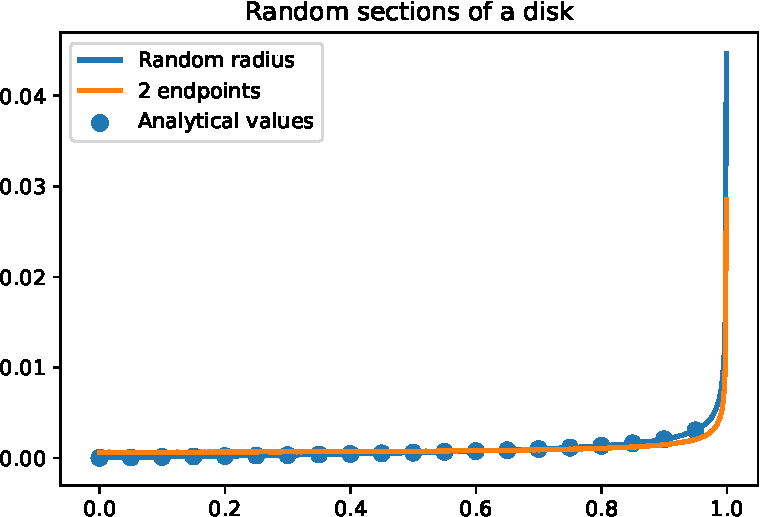
\includegraphics[width=.6\textwidth]{sections_disk-crop.pdf}%
 \label{fig:stereology:python:disk}%
\end{figure}

\begin{python}
import numpy as np
import matplotlib.pyplot as plt
N = 10000000;
nBins = 1000;
R = 1.;
# first simulation method: random radius
d = R * np.random.rand(N);
radii = np.sqrt(R**2 - d**2);
probaSimu = np.histogram(radii, bins=nBins);
plt.plot(probaSimu[1][:-1], probaSimu[0]/N, linewidth=2);
\end{python}

The second method consists in choosing 2 random points on the circle, given by two random angles.
\begin{python}
#2nd method: random points on the circle
# from 2 random angles
theta = np.pi*2*np.random.rand(int(N),2);
dX = np.diff(R * np.cos(theta))
dY = np.diff(R * np.sin(theta));
radii = 1./2 * np.sqrt(dX**2 + dY**2);
probaSimu2 = np.histogram(radii, bins=nBins);
plt.plot(probaSimu2[1][:-1], probaSimu2[0]/N, linewidth=2);
\end{python}

Finally, the analytical results are computed for comparison.
\begin{python}
# analytical values
step = .05;
r2 = np.arange(0, R, step);
probaReal = 1./R * r2 / np.sqrt(R**2-r2**2);
probaReal = probaReal * R / nBins; # approximation of the integral
plt.scatter(r2, probaReal, 50);
# display results
plt.legend(["Unique random points", "2 random points", "Analytical values"])
plt.show()
plt.savefig('sections_disk.pdf')
\end{python}
\vspace*{-8pt}
\subsection{Random planar sections of a sphere}
\vspace*{-8pt}
\begin{figure}[H]
 \centering\caption{Simulations of random chords of a sphere.}%
 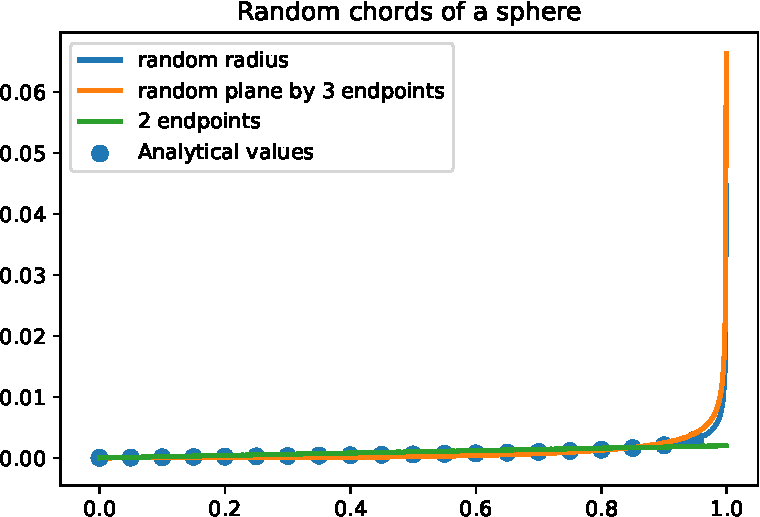
\includegraphics[width=.6\textwidth]{sections_sphere-crop.pdf}%
 \label{fig:stereology:python:sphere}%
\end{figure}

\begin{python}
import numpy as np
import matplotlib.pyplot as plt

def generatePointsOnSphere(nb_points, R):
    """
    Generate points on a sphere
    @param nb_points: number of points
    @return n: array of size nb_points x 3
    """
    n = np.random.randn(nb_points, 3);
    mynorm = np.linalg.norm(n, axis=1);
    n = R * n / np.transpose(np.matlib.repmat(mynorm, 3, 1));
    
    return n

def dot(A, B, ax=1):
    """ dot product for arrays
    """
    return np.sum(A.conj()*B, axis=ax );
\end{python}

\subsubsection{First simulation: random radius}

This method is equivalent to the first case of the disk chord. The 3D property of the sphere is not used and thus the code is strictly equivalent to the 2D case.

\begin{python}
# initial values	 
N = 1e7;      # number of samples, float number
R = 1;        # radius of the sphere
nBins = 1000; # number of bins for histogram computation
# first simulation method: random radius
d = R * np.random.rand(int(N));
radii = np.sqrt(R**2 - d**2);
probaSimu = np.histogram(radii, bins=nBins);
plt.plot(probaSimu[1][:-1], probaSimu[0]/N, linewidth=2);
\end{python}

\subsubsection{Second simulation: 3 endpoints}
Define a random plane from 3 points randomly chosen on the sphere. Let $n_1$, $n_2$ and $n_3$ be 3 points on the sphere. These points define the plane $\mathcal{P}$.
The distance between the center of the sphere $O$ and the plane $\mathcal{P}$ is given by the relation:
$$d(0, \mathcal{P})=\frac{|\vec{n}\cdot\vec{u}|}{||\vec{n}||}$$
with $\vec{u}=\vec{n_2}-\vec{n_1}$, $\vec{v}=\vec{n_3}-\vec{n_1}$, and $\vec{n}=\vec{u} \wedge\vec{v}$ the normal vector to the plane. The results are presented in Fig. \ref{fig:stereology:python:sphere}.

This is a case of Bertrand's paradox: the definition of randomness is not good in the present case.
\begin{python}
# second simulation
# choose 3 points to define a plane,
# then, compute the distance from the origin to this plane
n1 = generatePointsOnSphere(N, R);
n2 = generatePointsOnSphere(N, R);
n3 = generatePointsOnSphere(N, R);
# u and v belong to the plane
u=n2-n1;
v=n3-n1;
# n: normal vector to the plane
n=np.cross(u,v);
x = dot(n, n1) / np.linalg.norm(n, axis=1);
# distance from the origin to the plane:
r = np.sqrt(R**2 - x**2);
probaSimu = np.histogram(r, bins=nBins);
plt.plot(probaSimu[1][:-1], probaSimu[0]/N, linewidth=2);
\end{python}

\subsubsection{3rd simulation: 2 endpoints}
This situation presents the random choice of two points on the sphere, and the computation of their distance. This produces a linear probability (see Fig.\ref{fig:stereology:python:sphere}).
\begin{python}
# 3rd case: 
# 2 points on the sphere and distance between them
n1 = generatePointsOnSphere(N);
n2 = generatePointsOnSphere(N);
r = 1./2 * np.linalg.norm(n1-n2, axis=1);
probaSimu = np.histogram(r, bins=nBins);
plt.plot(probaSimu[1][:-1], probaSimu[0]/N, linewidth=2);
\end{python}

\subsubsection{Analytical values}
This code evaluates analytical values.

\begin{python}
# analytical values
step = .05;
r2 = np.arange(0, R, step);
probaReal = 1./R * r2 / np.sqrt(R**2-r2**2);
probaReal = probaReal * R / nBins; # approximation of the integral
plt.scatter(r2, probaReal, 50);

# display
plt.legend(["random plane by 3 points on the sphere", "2 points on the sphere", "Analytical values"])
plt.show();
plt.savefig("section_sphere.pdf") # save as pdf file
\end{python}

The results are displayed in Fig. \ref{fig:stereology:python:sphere}.

\begin{note}The Bertrand's paradox is illustrated by the fact that ``at random'' can provide several different interpretations. 
The objective here is to focus on the computational choices that can be made in order to provide random chords or random points on a sphere.\end{note}
